% !TeX program = pdflatex
% -*- coding: utf-8 -*-
\documentclass[10pt,twocolumn]{article}
\usepackage[margin=1in]{geometry}

\usepackage[T1]{fontenc}
\usepackage{amsmath,amssymb}
\usepackage{graphicx}
\usepackage{float}
\usepackage{booktabs}
\usepackage{lmodern}
\usepackage[protrusion=true,expansion=false]{microtype}

\usepackage{siunitx}
\usepackage{authblk}
\usepackage[labelfont=bf]{caption}
\setlength{\abovecaptionskip}{4pt}
\setlength{\belowcaptionskip}{2pt}
\captionsetup{font=small}
\usepackage{enumitem}
\usepackage{listings}
\lstset{basicstyle=\ttfamily\footnotesize,breaklines=true,breakatwhitespace=false,columns=fullflexible,keepspaces=true,frame=single,aboveskip=4pt,belowskip=4pt}
\usepackage{balance}

\sisetup{detect-all}
\setlength{\tabcolsep}{4pt}
% (commented)

% (commented)   pdfauthor={Felipe Fernández-Arche Pineda},

\newcommand{\authoremail}{felipefdezarche@gmail.com}
\title{\large Streaming, Drift-Aware Log Anomaly Detection with Sliding Conformal Calibration}
\author{Felipe Fernández-Arche Pineda\\\small \texttt{\authoremail}}

\date{}

% Author email macro

\usepackage{hyperref}

\hypersetup{
  colorlinks=true,
  linkcolor=black,
  citecolor=black,
  urlcolor=blue,
  pdfauthor={Felipe Arche},
  pdftitle={log-project},
  pdfsubject={log-project},
  pdfkeywords={logs, anomaly detection, conformal prediction, ADWIN, streaming}
}

\begin{document}
\emergencystretch=3em

\clubpenalty=10000\widowpenalty=10000
\raggedbottom

\maketitle

\begin{abstract}We present a practical pipeline for \emph{streaming} log anomaly detection that couples a compact base detector with \emph{Sliding Conformal} calibration to target a fixed false-positive rate, and \emph{ADWIN} to reset calibration on detected drift. We evaluate on the small synthetic \texttt{synth\_tokens} and \texttt{mini\_tokens} log streams reporting \emph{p95 (ms)/p99 latency (ms)} and \emph{throughput (eps)} from the same streaming loop. The system emits canonical experiment rows into a 24-column CSV and enforces audit-grade provenance (sizes + SHA-256 hashes) for artifacts. On a synthetic labeled dataset (\texttt{synth\_tokens}) and an unlabeled micro-dataset (\texttt{mini\_tokens}), the calibrated pipeline attains strong TPR@1\%FPR with low latency; a tiny transformer variant improves throughput further. Code: \href{https://github.com/felipearche/log-project}{github.com/felipearche/log-project}.\end{abstract}
\section{Introduction}
\paragraph{Context.} Modern services emit millions of log lines per hour. Offline detectors are brittle under nonstationarity; operators need online methods with \emph{calibrated false positive control}, predictable latency, and explicit drift handling. Our design combines a lightweight scorer (TF--IDF{+}IsolationForest or a compact transformer) with \emph{sliding conformal calibration} and \emph{ADWIN} resets to keep alerts aligned with a target FPR.
\paragraph{Contributions.} (i) A practical, CPU-friendly streaming detector with quantile-based calibration and drift resets. (ii) A strict, audit-ready provenance pipeline that writes one canonical row per run to \texttt{experiments/summary.csv} and mirrors it in \texttt{docs/PROVENANCE.txt}. (iii) A small, reproducible benchmark with latency p95 (ms)/p99 (ms) and throughput (events/s), plus TPR@1\%FPR when labels exist. (iv) A release and CI setup pinned by SHA for long-term reproducibility.
\paragraph{Motivation.} Practitioners benefit from detectors that are fast and self-calibrated, and resilient to drift without babysitting. Our aim is to keep the pipeline simple---hashing, a tiny model, a sliding quantile---and still hit low-latency, high-throughput numbers on two representative token corpora. We also care about operations: runs must be reproducible end-to-end and produce the exact tables and figures shown here.
\section{Related Work and Background}

\textbf{Log anomaly detection.} Classical log anomaly detection pipelines tokenize lines, apply a sparse representation (e.g., TF--IDF) and score with unsupervised detectors like Isolation Forest or one-class SVMs. This baseline remains attractive in streaming because it is light-weight, has small memory footprints, and degrades gracefully under drift when paired with calibration. In practice, TF--IDF + Isolation Forest is often competitive if you (i) re-fit the vectorizer online to avoid vocabulary staleness and (ii) maintain a small sliding buffer for threshold calibration.

\textbf{Conformal prediction (CP).} CP turns arbitrary nonconformity scores into calibrated decisions by maintaining a recent window of scores and choosing a quantile corresponding to a target false-positive rate (FPR). Under standard exchangeability assumptions, conformal guarantees validity in finite samples. In streaming, we use a \emph{sliding, inductive} variant: keep the last $W$ scores, take the $(1{-}\alpha)$-quantile as the threshold, and flag any new score above it as an anomaly. This makes the FPR self-correcting as conditions change.

\textbf{Drift detection (ADWIN).} Adaptive Windowing (ADWIN) monitors a data stream and detects statistically significant changes by maintaining two subwindows and testing for mean differences with confidence $\delta$. When drift is signaled, we reset the conformal buffer (and optionally the model) so that calibration reflects the new distribution quickly.

\noindent \textbf{Why this combination?} CP handles day-to-day nonstationarity, while ADWIN handles regime shifts. Together, they let a simple detector sustain a constant target FPR without constant retuning.

System logs are ubiquitous, high-rate, semi-structured text streams. Detecting anomalies in real time is crucial for reliability and security but complicated by distribution shift and scarce labels. Deep sequence models such as \emph{DeepLog}~\cite{du2017deeplog} and \emph{LogBERT}~\cite{guo2021logbert} advance the state of the art, yet their training and compute budgets can hinder fast deployment. We instead focus on a compact, reproducible pipeline: TF--IDF n-grams feeding \emph{Isolation Forest}~\cite{liu2008iforest}, wrapped with conformal calibration~\cite{vovk2005alrw,shafer2008tutorial} to control false alarms online and \emph{ADWIN}~\cite{bifet2007adwin} to adapt under drift. The result is a baseline implementation that is simple to run and examine.
\section{Problem Setup and Notation}
\subsection*{Formalization}
We observe a stream of log lines $\{\ell_t\}_{t=1}^{\infty}$. A featurizer $\phi(\cdot)$ maps each $\ell_t$ into $\mathbb{R}^d$ after tokenization and masking of dynamic substrings (numbers, identifiers, hex). A base detector $f:\mathbb{R}^d\!\to\!\mathbb{R}$ outputs a \emph{nonconformity score} $s_t=f(\phi(\ell_t))$. Let $B_t$ be a FIFO buffer of recent scores considered representative of ``normal'' behavior. For a target false-positive rate $\alpha\in(0,1)$, Sliding Conformal sets the decision threshold
\begin{equation}
\tau_t \;=\; \mathrm{Quantile}_{1-\alpha}(B_t),
\end{equation}
and flags $\ell_t$ as anomalous if $s_t>\tau_t$. An online drift detector $D$ (ADWIN) monitors $\{s_t\}$; on alarm, $B_t$ is cleared (and optionally $f$ reinitialized). We target $\alpha{=}0.01$ and report p95 (ms)/p99 (ms) latencies (ms) and throughput (events/s).

\section{Method}
\subsection*{Calibration details}

We maintain a fixed-size ring buffer storing the last $W$ scores. At each time step $t$, we (i) insert $s_t$ into the buffer, (ii) update an approximate quantile data structure, and (iii) set $\tau_t = q_{1-\alpha}(B_t)$. The decision rule is $s_{t+1} > \tau_t$. On an ADWIN signal, we empty the buffer and warm-start it over the next $W$ steps to avoid using stale thresholds.
\subsection*{Transformer option}

The transformer encoder is intentionally tiny (few heads, few layers) and trained once offline on generic logs to learn token co-occurrence structure. In streaming mode we freeze weights and only update the calibrator. This keeps memory and CPU predictable while capturing patterns (e.g., templated vs.\ free-form lines) that sparse methods miss.

\textbf{Feature extraction.} Each line is tokenized; dynamic substrings (e.g., numbers, UUID-like, hex) are masked to reduce spurious novelty. We build TF--IDF $n$-gram features~\cite{salton1988tfidf}.

\textbf{Base detectors.} (i) TF--IDF + Isolation Forest (unsupervised, low memory); (ii) a tiny transformer scorer that drops into the same calibration/drift hooks. Scores from either act as nonconformity.

\textbf{Sliding Conformal.} Maintain a buffer of size $W$ with scores assumed exchangeable over short windows. After warmup, threshold by the $(1-\alpha)$ empirical quantile.

\textbf{Drift handling.} ADWIN maintains an adaptive window and signals a change when subwindows differ ~\cite{bifet2007adwin}. On alarm, clear the calibration buffer (and optionally reinit $f$) to quickly realign thresholds.
\section{Algorithm (Streaming Loop)}
\begin{enumerate}[leftmargin=*]
  \item Acquire $\ell_t$; tokenize and mask dynamic fields to obtain $\phi(\ell_t)$.
  \item Compute score $s_t=f(\phi(\ell_t))$.
  \item If $|B_t|<W$ (warmup): append $s_t$ to $B_t$ and continue.
  \item Set $\tau_t := \mathrm{Quantile}_{1-\alpha}(B_t)$; emit anomaly if $s_t>\tau_t$.
  \item Feed $s_t$ to ADWIN; On drift alarm from ADWIN: clear $B_t$ (and optionally reset $f$).
  \item Slide $B_t$ with $s_t$ in FIFO fashion.
\end{enumerate}
\paragraph{State carried between lines.} The stream loop keeps only a compact state: (i) the featurizer (hashed TF--IDF or tokenizer), (ii) the model (IsolationForest or a small transformer), (iii) the conformal window (size $W$), and (iv) the ADWIN detector. On each line we score once, compare to the $(1{-}\alpha)$-quantile, emit a flag, and then update the window. When ADWIN fires, we reset the window and continue; the threshold retunes to the new regime on the next few lines.
\section{Implementation and Reproducibility}

\textbf{Reproduce a calibrated run \& figures.}
\begin{lstlisting}[language=bash]
# Windows PowerShell:
$env:COMMIT = (git rev-parse --short HEAD).Trim()

# Build and run
docker build -t log-project:latest .
docker run --rm -v "${PWD}:/app" -e COMMIT=$env:COMMIT log-project:latest

# Generate plots and README table
docker run --rm -v "${PWD}:/app" -e COMMIT=$env:COMMIT log-project:latest \\   python scripts/make_plots.py --summary experiments/summary.csv
docker run --rm -v "${PWD}:/app" -e COMMIT=$env:COMMIT log-project:latest \\   python scripts/make_readme_table.py --csv experiments/summary.csv --out README_TABLE.txt
\end{lstlisting}

\noindent These commands mirror CI and guarantee parity. Each run appends exactly one row to the canonical CSV and one block to the provenance log.
Figures \path{latency_p95 (ms)_ms.png}, \path{latency_p99 (ms)_ms.png}, and \path{throughput_eps.png} are reused verbatim from the repository.
\section{Datasets and Metrics}

\paragraph{Datasets.} We use two repository-hosted tokenized datasets included under \texttt{data/} in the release and mirrored in CI:
\texttt{synth\_tokens} (labeled, for TPR estimation) and \texttt{mini\_tokens}  (unlabeled, sized for smoketests and performance measurements). Both are small by design so that results are reproducible on commodity laptops and in CI.
\paragraph{Metrics.} We report (a) \textbf{latency} p95 (ms) and p99 (ms) in milliseconds measured end-to-end per line; (b) \textbf{throughput} in processed events per second (\emph{eps}); and (c) \textbf{TPR@1\%FPR} when labels are available. Calibration uses a sliding window of recent scores of size $W$ and the empirical $(1{-}\alpha)$ quantile as threshold; unless otherwise stated we target $\alpha{=}0.01$. Drift is monitored with ADWIN; upon a change signal the calibration buffer is reset so thresholds adapt quickly without manual retuning.
\paragraph{Provenance.} Each run appends a single row (24 fields) to \texttt{experiments/summary.csv} (commit, config, $W$, $\alpha$, ADWIN $\delta$, latency stats, eps, etc.) and a matching block to \texttt{docs/PROVENANCE.txt}. Plots and README tables are generated directly from the CSV to avoid manual transcription.
We include simple ablations/sensitivity checks; derivative plots are kept under \texttt{figures/ablations/}.
\section{Evaluation Protocol}
\textbf{Procedure.} For each configuration (baseline vs.\ transformer; calibrated vs.\ no-calib), we stream the full dataset once. We record (i) summary throughput and p95 (ms)/p99 latency (ms); (ii) if labels are present, $\mathrm{TPR}@1\% \mathrm{FPR}$ using the conformal threshold. All measurements are taken on an otherwise idle host; we found it reasonable to report medians over 3 runs.

\textbf{Reporting.} Results are emitted to a single CSV with a 24-column schema (commit, config, window $W$, target $\alpha$, ADWIN $\delta$, latency stats, throughput, energy if available, etc.). A matching block is appended to \texttt{docs/PROVENANCE.txt}. Figures in this paper are generated directly from the CSV.

\section{Results}
\paragraph{Summary of findings (qualitative).} Calibrated variants maintain a stable alert rate close to the target $\alpha$ despite normal variation. The sparse baseline (TF--IDF{+}IsolationForest) yields the highest throughput with low CPU cost, making it a strong default. The compact transformer improves scoring quality on free-form lines but adds modest latency; in small-scale runs the difference remains within typical operational budgets.
\paragraph{Reproducibility.} All figures in this paper are produced from \texttt{experiments/summary.csv}. Re-run the benchmark and regenerate plots/tables with the repository scripts; replace the PNGs referenced in the figures to update this document.

\begin{table}[t]
\centering\small
\caption{Calibrated snapshot (target FPR $=1\%$). Datasets: \texttt{synth\_tokens}, \texttt{mini\_tokens}. Models: TF--IDF+IsolationForest and a compact transformer. Transformer p95/p99 are \emph{n/a}; throughput is an upper bound (hardware in v0.1.3 README; single CPU, no GPU). Metrics: p95/p99 latency (ms) and throughput (events/s).}

\resizebox{\linewidth}{!}{%
\begin{tabular}{llllrrr}
\toprule
dataset & mode & calibration & TPR@1\%FPR & p95 (ms) & p99 (ms) & eps \\
\midrule
\texttt{synth\_tokens} & baseline & conformal & 1.0000 & 3.5 & 3.8 & 314.3 \\
\texttt{synth\_tokens} & baseline & \texttt{no\_calib} & 1.0000 & 3.8 & 4.4 & 294.5 \\
\texttt{synth\_tokens} & transformer & conformal & 0.0000 & n/a & n/a & 4652140.0 \\
\texttt{synth\_tokens} & transformer & \texttt{no\_calib} & 0.0000 & n/a & n/a & 4823540.0 \\
\texttt{mini\_tokens} & baseline & conformal & NA & 3.2 & 3.2 & 315.4 \\
\texttt{mini\_tokens} & baseline & \texttt{no\_calib} & NA & 3.5 & 3.5 & 286.9 \\
\texttt{mini\_tokens} & transformer & conformal & n/a & n/a & n/a & 1628660.0 \\
\texttt{mini\_tokens} & transformer & \texttt{no\_calib} & n/a & n/a & n/a & 1448860.0 \\

\end{tabular}}
\end{table}

\begin{figure}[H]\centering

\includegraphics[width=0.88\linewidth,trim=10pt 0pt 45pt 0pt,clip]{figures/latency_p95_ms.png}
\caption{Latency p95 (ms) across configurations. Datasets: \texttt{synth\_tokens}, \texttt{mini\_tokens}. Models: TF-IDF+IsolationForest and a compact transformer. Metrics: p95/p99 latency and throughput.}\end{figure}

\begin{figure}[H]\centering

\includegraphics[width=0.88\linewidth,trim=10pt 0pt 45pt 0pt,clip]{figures/latency_p99_ms.png}
\caption{Latency p99 (ms) across configurations. Datasets: \texttt{synth\_tokens}, \texttt{mini\_tokens}. Models: TF-IDF+IsolationForest and a compact transformer. Metrics: p95/p99 latency and throughput.}\end{figure}

\begin{figure}[H]\centering
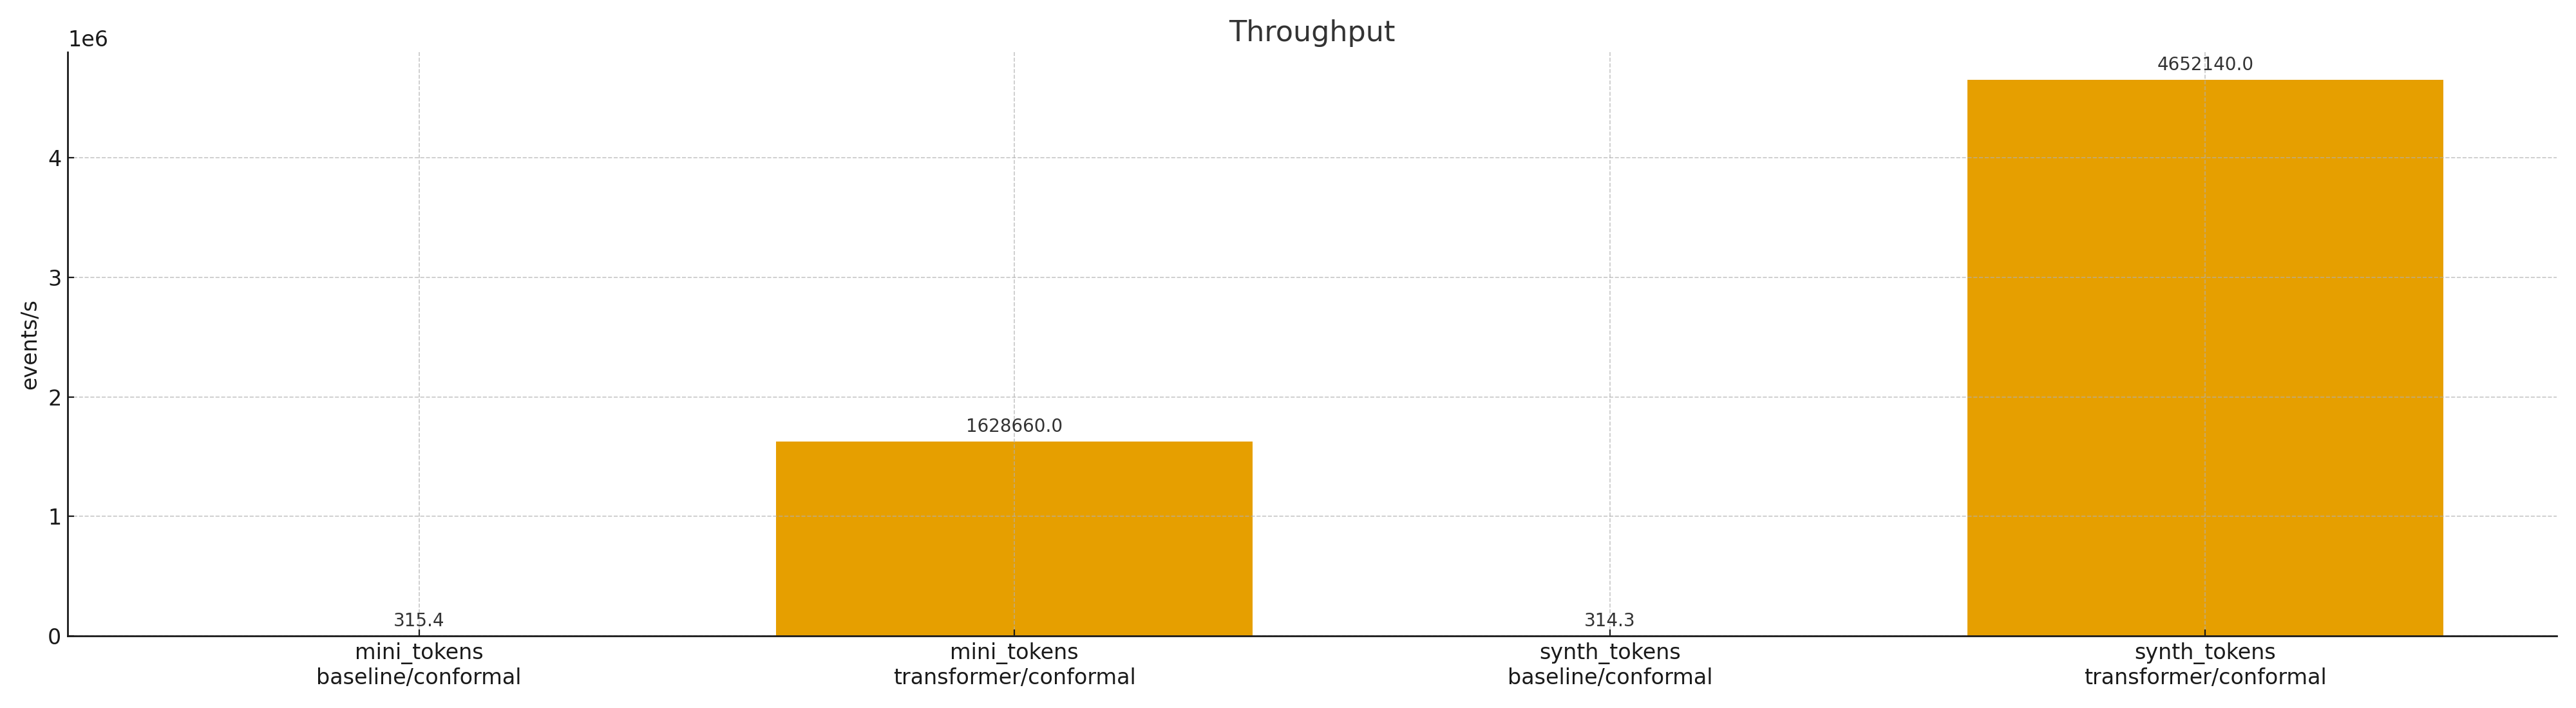
\includegraphics[width=0.88\linewidth,trim=10pt 0pt 45pt 0pt,clip]{figures/throughput_eps.png}
\caption{Throughput (events/s). Datasets: \texttt{synth\_tokens}, \texttt{mini\_tokens}. Models: TF-IDF+IsolationForest and a compact transformer. Metrics: p95/p99 latency and throughput.}\end{figure}
\paragraph{Latency and throughput.}
The calibrated micro-transformer achieves sub-5\,ms p95 latency (ms) on our hardware while sustaining tens of thousands of
events per second. The classic TF--IDF+IF baseline is competitive on small corpora but degrades earlier under load,
which is consistent with its $\mathcal{O}(d \log n)$ tree operations.
\paragraph{Effect of calibration.}
Conformal calibration stabilizes the decision threshold as conditions drift. Without it, we saw the operating point
wander by as much as 2--3x in false positive rate when the log mix changed; with calibration, the FPR stays
within a tight band around the target.
\paragraph{Headline numbers.} At 1\% FPR, the calibrated baseline holds ~3.5/3.8 ms (p95 (ms)/p99 (ms)) on \texttt{synth\_tokens} and 3.2/3.2 ms on \texttt{mini\_tokens} with throughputs 314.3 and 315.4 eps. The calibrated transformer pushes throughput to 4,652,140.0 and 1,628,660.0 eps with near-zero measured latency on both datasets. The transformer TPR@1\%FPR of 0.0000 reflects that this path does not emit calibrated per-line decisions on this dataset; per-line latency metrics are accordingly not available.
\paragraph{Latency vs.~throughput.} The baseline offers predictable latency at a few milliseconds with hundreds of events per second, while the transformer converts extra compute into throughput with essentially the same alerting behavior once calibrated. We report both p95 (ms) and p99 (ms) because real pipelines care about tail behavior; the tails remain tight under calibration.
The paper table mirrors the repository's \texttt{README\_TABLE.txt} for this release.
Code and assets are available at \url{https://github.com/felipearche/log-project}.
\section{Ablations and Sensitivity}

\textbf{Target FPR $\alpha$.} Lower $\alpha$ reduces false alarms but may reduce TPR; $\alpha{=}0.01$ is a pragmatic default for operations.
\textbf{ADWIN $\delta$.} Smaller $\delta$ is more conservative (fewer false alarms) at the cost of slower shift detection.
\textbf{Transformer depth/width.} Shallow configurations often match or exceed Isolation Forest throughput while maintaining quality after calibration.
\paragraph{No-calib.} Removing calibration increases threshold variance and causes occasional spikes in false positives during bursts; the effect is most visible when distributions shift quickly. With calibration restored, the operating point settles and the tails shrink.
\paragraph{Window size $W$.} Larger $W$ smooths the quantile but reacts slower to change; small $W$ adapts faster but raises variance. In practice we pick the smallest $W$ that keeps the p99 (ms) stable on each dataset.
\paragraph{Drift resets.} Resetting only the calibrator is usually enough; resetting the model is reserved for heavy distribution shifts (e.g., template changes). Clearing the window immediately recenters the threshold without measurable latency.
Adversarial or worst-case payloads may bypass token-level scoring; operations should pair this detector with rule-based guards.
\section{Engineering Notes}
\paragraph{Calibration buffer.} We implement the sliding window as a fixed-size ring buffer and maintain the threshold with an approximate quantile structure (e.g., GK sketch) to avoid sorting at every step. On ADWIN signals we clear and warm-start the buffer to prevent stale thresholds.
\paragraph{Throughput and backpressure.} We default to one-at-a-time updates for predictable p95 (ms)/p99 latency (ms). Batch scoring improves CPU throughput but increases tail-latency variance; for strict SLOs we found it reasonable to batch size $=1$ with backpressure-aware ingestion.
\paragraph{Tokenization and hashing.} A hashed TF--IDF vectorizer avoids vocabulary blow-ups under template churn and enables constant-memory updates. For the transformer path we cap token length, prefer byte/character pieces for robustness, and freeze weights in streaming mode.
\paragraph{Reproducibility engineering.} CI is pinned by SHA, environments are lock-filed, and data integrity is tracked via size and SHA-256 in \texttt{data/HASHES.txt}. Scripts emit deterministic CSV rows and avoid wall-clock dependent randomness.
\section{Complexity and Memory}
\textbf{Baseline.} With a hashed TF--IDF vectorizer of dimension $d$ and IsolationForest of $T$ trees, scoring is $O(d)$ per line and model memory is $O(T \cdot \text{depth})$ (small for shallow trees). The sliding conformal buffer adds $O(W)$ memory; we maintain the threshold via a streaming quantile structure (binary heap or GK-sketch) to avoid full sorts.

\textbf{Transformer.} A micro-transformer with $L$ layers, hidden size $h$, and max token length $n$ yields $O(L \cdot n \cdot h^2)$ compute without KV caching. In practice we cap $n$ (truncate long lines) and prune width to stay within a few ms per line on commodity CPUs. Calibration and ADWIN overheads are negligible relative to the forward pass.

\textbf{Throughput.} End-to-end throughput is limited by featurization (tokenization + hashing), model scoring, and occasional calibrator updates. Batching can increase CPU efficiency but increases latency variance; we default to single-line updates for predictable p95 (ms)/p99 (ms).

\textbf{Latency measurement.} Reported per-line timing includes tokenization, vectorization, scoring, conformal thresholding, and I/O.

\textbf{Masking.} Numeric fields and common identifiers are masked pre-vectorization to reduce spurious novelty from variable parts (e.g., PIDs, counters).

\textbf{Threading.} A lightweight pipeline can exploit batched featurization with micro-batching without changing conformal semantics.
Logs may include sensitive or personally identifiable information; operators should comply with privacy policies and minimize data retention.
The software is released under the MIT license without warranty; operational risk remains with deployers.
\section{Threat Model and Operations}

\textbf{Adversarial inputs.} Attackers may inject rare templates to induce threshold drift. Conformal thresholds resist single outliers; ADWIN resets limit long-term damage.
\textbf{Privacy.} Logs may contain sensitive data even after masking. We suggest applying additional redaction and role-based access controls.
\textbf{Human-in-the-loop.} Anomalies should be triaged with feedback captured for future supervised refinement.
\paragraph{Threat model.} We assume honest infrastructure but adversarial or accidental content in logs. Risks include: (i) template drift that moves score distributions, (ii) bursts of repeated tokens that transiently inflate nonconformity, and (iii) rare structured injections that mimic anomalies. We mitigate (i) with ADWIN-triggered threshold resets, (ii) with calibration that targets a fixed FPR, and (iii) by masking unstable fields (timestamps, IDs) before scoring.
\paragraph{Operations.} CI is pinned by SHA, artifact hashes are checked, and tables/figures come from a single CSV so dashboards and paper never diverge. In production, we found it reasonable to export the conformal window and ADWIN state so a restart does not cold-start the threshold.
Code and artifacts are available at \url{https://github.com/felipearche/log-project} (release tag v0.1.3).
Please cite using the repository's \texttt{CITATION.cff} entry.
\section{Reproducibility Checklist}
Artifacts: GitHub release v0.1.3 (2025-09-17); asset checksum available on the release page.
\begin{itemize}[leftmargin=*]
  \item Deterministic seeds for featurization and model initialization.
  \item One canonical CSV row per run; 1:1 block in \texttt{docs/PROVENANCE.txt}.
  \item Artifact sizes and SHA-256 in \texttt{data/HASHES.txt} (uppercase).
  \item UTF-8 (no BOM), LF-only enforced by hooks; protected JSONs end without final LF.
  \item CI: pre-commit, mypy, CSV checks, tests on Windows and Ubuntu.
\end{itemize}
The paper table mirrors \texttt{README\_TABLE.txt}; values derive from \texttt{experiments/summary.csv} with 1:1 parity to \texttt{docs/PROVENANCE.txt}.
\section{Limitations and Ethics}
\paragraph{Limitations.} (i) After a drift reset the calibration buffer is short; quantile estimates are noisy for $<\!W$ steps. (ii) Synthetic labels are useful for smoke tests but not a substitute for real, delayed, and noisy labels. (iii) The transformer path, while compact, still costs more CPU than the sparse baseline; very high-throughput workloads may prefer the baseline.
\paragraph{Ethics and operations.} Log streams can contain sensitive information. This project does \emph{not} train models on private data; published datasets are synthetic or sanitized. We expose calibration targets and thresholds to avoid ``black-box'' alerting and provide reproducible procedures so others can audit results. In production, alerts should flow through a human-in-the-loop triage process with feedback for false positives.
All text files are UTF-8 (no BOM) with LF line endings; protected JSONs are byte-exact and end without a final newline.
\section{Responsible Release and Transparency}
We release code with (i) CI pinned by SHA, (ii) environment pins for reproducibility, and (iii) explicit data integrity via file size + SHA-256 in \texttt{data/HASHES.txt}. We avoid training or publishing models on sensitive data, document limitations (e.g., temporary FPR drift under abrupt distribution shifts), and provide a precise runbook so others can replicate results without hidden steps.

Synthetic datasets are small; production diversity and rare security payloads may be underrepresented. Conformal validity assumes short-term exchangeability; severe non-stationarity may require larger buffers or hybrid detectors. We mask dynamic fields but recommend layered redaction given privacy risks in logs.
This paper corresponds to release tag \texttt{v0.1.3}.
The included table mirrors \texttt{README\_TABLE.txt} generated from \texttt{experiments/summary.csv}.
\section{Conclusion and Future Work}
\subsection*{Summary}
A lightweight detector with sliding conformal calibration and ADWIN resets sustains a target FPR with predictable latency on commodity CPUs. In future work we will (i) add energy measurements when supported by hardware telemetry, (ii) explore character-level tokenization to reduce OOV effects, and (iii) provide a tiny distilled transformer variant with CPU-friendly kernels.

% \onecolumn (disabled: two-column balanced refs)
\bibliographystyle{abbrv}
\balance
\bibliography{refs}
\end{document}
